%======================================================================
% University of Waterloo Thesis Template for LaTeX 
% Last Updated August 21, 2018 
% by Stephen Carr, IST Client Services, 
% University of Waterloo, 200 University Ave. W., Waterloo, Ontario, Canada
% FOR ASSISTANCE, please send mail to rt-IST-CSmathsci@rt.uwaterloo.ca

% DISCLAIMER
% To the best of our knowledge, this template satisfies the current uWaterloo thesis requirements.
% However, it is your responsibility to assure that you have met all 
% requirements of the University and your particular department.

% Many thanks for the feedback from many graduates who assisted the development of this template.
% Also note that there are explanatory comments and tips throughout this template.
%======================================================================
% Some important notes on using this template and making it your own...

% The University of Waterloo has required electronic thesis submission since October 2006. 
% See the uWaterloo thesis regulations at
% https://uwaterloo.ca/graduate-studies/thesis.
% This thesis template is geared towards generating a PDF 
% version optimized for viewing on an electronic display, including 
% hyperlinks within the PDF.

% DON'T FORGET TO ADD YOUR OWN NAME AND TITLE in the "hyperref" package
% configuration below. THIS INFORMATION GETS EMBEDDED IN THE PDF FINAL PDF DOCUMENT.
% You can view the information if you view properties of the PDF document.

% Many faculties/departments also require one or more printed
% copies. This template attempts to satisfy both types of output. See additional notes below.
% It is based on the standard "book" document class which provides all necessary 
% sectioning structures and allows multi-part theses.

% If you are using this template in Overleaf (cloud-based collaboration service), then it is 
% automatically processed and previewed for you as you edit.

% For people who prefer to install their own LaTeX distributions on their own computers, and process 
% the source files manually, the following notes provide the sequence of tasks:
 
% E.g. to process a thesis called "mythesis.tex" based on this template, run:

% pdflatex mythesis	-- first pass of the pdflatex processor
% bibtex mythesis	-- generates bibliography from .bib data file(s)
% makeindex         -- should be run only if an index is used 
% pdflatex mythesis	-- fixes numbering in cross-references, bibliographic references, glossaries, index, etc.
% pdflatex mythesis	-- it takes a couple of passes to completely process all cross-references

% If you use the recommended LaTeX editor, Texmaker, you would open the mythesis.tex
% file, then click the PDFLaTeX button. Then run BibTeX (under the Tools menu).
% Then click the PDFLaTeX button two more times. If you have an index as well,
% you'll need to run MakeIndex from the Tools menu as well, before running pdflatex
% the last two times.

% N.B. The "pdftex" program allows graphics in the following formats to be
% included with the "\includegraphics" command: PNG, PDF, JPEG, TIFF
% Tip 1: Generate your figures and photos in the size you want them to appear
% in your thesis, rather than scaling them with \includegraphics options.
% Tip 2: Any drawings you do should be in scalable vector graphic formats:
% SVG, PNG, WMF, EPS and then converted to PNG or PDF, so they are scalable in
% the final PDF as well.
% Tip 3: Photographs should be cropped and compressed so as not to be too large.

% To create a PDF output that is optimized for double-sided printing: 
%
% 1) comment-out the \documentclass statement in the preamble below, and
% un-comment the second \documentclass line.
%
% 2) change the value assigned below to the boolean variable
% "PrintVersion" from "false" to "true".

%======================================================================
%   D O C U M E N T   P R E A M B L E
% Specify the document class, default style attributes, and page dimensions, etc.
% For hyperlinked PDF, suitable for viewing on a computer, use this:
\documentclass[letterpaper,12pt,titlepage,oneside,final]{book}
 
% For PDF, suitable for double-sided printing, change the PrintVersion variable below
% to "true" and use this \documentclass line instead of the one above:
%\documentclass[letterpaper,12pt,titlepage,openright,twoside,final]{book}

% Some LaTeX commands I define for my own nomenclature.
% If you have to, it's easier to make changes to nomenclature once here than in a 
% million places throughout your thesis!
\newcommand{\package}[1]{\textbf{#1}} % package names in bold text
\newcommand{\cmmd}[1]{\textbackslash\texttt{#1}} % command name in tt font 
\newcommand{\href}[1]{#1} % does nothing, but defines the command so the
    % print-optimized version will ignore \href tags (redefined by hyperref pkg).
%\newcommand{\texorpdfstring}[2]{#1} % does nothing, but defines the command
% Anything defined here may be redefined by packages added below...

% This package allows if-then-else control structures.
\usepackage{ifthen}
\newboolean{PrintVersion}
\setboolean{PrintVersion}{false}
% CHANGE THIS VALUE TO "true" as necessary, to improve printed results for hard copies
% by overriding some options of the hyperref package, called below.

%\usepackage{nomencl} % For a nomenclature (optional; available from ctan.org)
\usepackage{amsmath,amssymb,amstext} % Lots of math symbols and environments
\usepackage[pdftex]{graphicx} % For including graphics N.B. pdftex graphics driver 

% Hyperlinks make it very easy to navigate an electronic document.
% In addition, this is where you should specify the thesis title
% and author as they appear in the properties of the PDF document.
% Use the "hyperref" package 
% N.B. HYPERREF MUST BE THE LAST PACKAGE LOADED; ADD ADDITIONAL PKGS ABOVE
\usepackage[pdftex,pagebackref=false]{hyperref} % with basic options
%\usepackage[pdftex,pagebackref=true]{hyperref}
		% N.B. pagebackref=true provides links back from the References to the body text. This can cause trouble for printing.
\hypersetup{
    plainpages=false,       % needed if Roman numbers in frontpages
    unicode=false,          % non-Latin characters in Acrobat’s bookmarks
    pdftoolbar=true,        % show Acrobat’s toolbar?
    pdfmenubar=true,        % show Acrobat’s menu?
    pdffitwindow=false,     % window fit to page when opened
    pdfstartview={FitH},    % fits the width of the page to the window
%    pdftitle={uWaterloo\ LaTeX\ Thesis\ Template},    % title: CHANGE THIS TEXT!
%    pdfauthor={Author},    % author: CHANGE THIS TEXT! and uncomment this line
%    pdfsubject={Subject},  % subject: CHANGE THIS TEXT! and uncomment this line
%    pdfkeywords={keyword1} {key2} {key3}, % list of keywords, and uncomment this line if desired
    pdfnewwindow=true,      % links in new window
    colorlinks=true,        % false: boxed links; true: colored links
    linkcolor=blue,         % color of internal links
    citecolor=green,        % color of links to bibliography
    filecolor=magenta,      % color of file links
    urlcolor=cyan           % color of external links
}
\ifthenelse{\boolean{PrintVersion}}{   % for improved print quality, change some hyperref options
\hypersetup{	% override some previously defined hyperref options
%    colorlinks,%
    citecolor=black,%
    filecolor=black,%
    linkcolor=black,%
    urlcolor=black}
}{} % end of ifthenelse (no else)

\usepackage[automake,toc,abbreviations]{glossaries-extra} % Exception to the rule of hyperref being the last add-on package
% If glossaries-extra is not in your LaTeX distribution, get it from CTAN (http://ctan.org/pkg/glossaries-extra), 
% although it's supposed to be in both the TeX Live and MikTeX distributions. There are also documentation and 
% installation instructions there.

% Setting up the page margins...
% uWaterloo thesis requirements specify a minimum of 1 inch (72pt) margin at the
% top, bottom, and outside page edges and a 1.125 in. (81pt) gutter
% margin (on binding side). While this is not an issue for electronic
% viewing, a PDF may be printed, and so we have the same page layout for
% both printed and electronic versions, we leave the gutter margin in.
% Set margins to minimum permitted by uWaterloo thesis regulations:
\setlength{\marginparwidth}{0pt} % width of margin notes
% N.B. If margin notes are used, you must adjust \textwidth, \marginparwidth
% and \marginparsep so that the space left between the margin notes and page
% edge is less than 15 mm (0.6 in.)
\setlength{\marginparsep}{0pt} % width of space between body text and margin notes
\setlength{\evensidemargin}{0.125in} % Adds 1/8 in. to binding side of all 
% even-numbered pages when the "twoside" printing option is selected
\setlength{\oddsidemargin}{0.125in} % Adds 1/8 in. to the left of all pages
% when "oneside" printing is selected, and to the left of all odd-numbered
% pages when "twoside" printing is selected
\setlength{\textwidth}{6.375in} % assuming US letter paper (8.5 in. x 11 in.) and 
% side margins as above
\raggedbottom

% The following statement specifies the amount of space between
% paragraphs. Other reasonable specifications are \bigskipamount and \smallskipamount.
\setlength{\parskip}{\medskipamount}

% The following statement controls the line spacing.  The default
% spacing corresponds to good typographic conventions and only slight
% changes (e.g., perhaps "1.2"), if any, should be made.
\renewcommand{\baselinestretch}{1} % this is the default line space setting

% By default, each chapter will start on a recto (right-hand side)
% page.  We also force each section of the front pages to start on 
% a recto page by inserting \cleardoublepage commands.
% In many cases, this will require that the verso (left-hand) page be
% blank, and while it should be counted, a page number should not be
% printed.  The following statements ensure a page number is not
% printed on an otherwise blank verso page.
\let\origdoublepage\cleardoublepage
\newcommand{\clearemptydoublepage}{%
  \clearpage{\pagestyle{empty}\origdoublepage}}
\let\cleardoublepage\clearemptydoublepage

% Define Glossary terms (This is properly done here, in the preamble and could also be \input{} from a separate file...)
% Main glossary entries -- definitions of relevant terminology
\newglossaryentry{computer}
{
name=computer,
description={A programmable machine that receives input data,
               stores and manipulates the data, and provides
               formatted output}
}

% Nomenclature glossary entries -- New definitions, or unusual terminology
\newglossary*{nomenclature}{Nomenclature}
\newglossaryentry{dingledorf}
{
type=nomenclature,
name=dingledorf,
description={A person of supposed average intelligence who makes incredibly brainless misjudgments}
}

% List of Abbreviations (abbreviations type is built in to the glossaries-extra package)
\newabbreviation{aaaaz}{AAAAZ}{American Association of Amateur Astronomers and Zoologists}

% List of Symbols
\newglossary*{symbols}{List of Symbols}
\newglossaryentry{rvec}
{
name={$\mathbf{v}$},
sort={label},
type=symbols,
description={Random vector: a location in n-dimensional Cartesian space, where each dimensional component is determined by a random process}
}
 
\makeglossaries

%======================================================================
%   L O G I C A L    D O C U M E N T
% The logical document contains the main content of your thesis.
% Being a large document, it is a good idea to divide your thesis
% into several files, each one containing one chapter or other significant 
% chunk of content, so you can easily shuffle things around later if desired.
%======================================================================
\begin{document}

%----------------------------------------------------------------------
% FRONT MATERIAL
% title page,declaration, borrowers' page, abstract, acknowledgements,
% dedication, table of contents, list of tables, list of figures, nomenclature, etc.
%----------------------------------------------------------------------
% T I T L E   P A G E
% -------------------
% Last updated June 14, 2017, by Stephen Carr, IST-Client Services
% The title page is counted as page `i' but we need to suppress the
% page number. Also, we don't want any headers or footers.
\pagestyle{empty}
\pagenumbering{roman}

% The contents of the title page are specified in the "titlepage"
% environment.
\begin{titlepage}
        \begin{center}
        \vspace*{1.0cm}

        \Huge
        {\bf Micromeda: a pathway prediction pipeline and web visualization tool for functional comparisons of microbial genomes and metagenome-assembled genomes}

        \vspace*{1.0cm}

        \normalsize
        by \\

        \vspace*{1.0cm}

        \Large
        Lee Bergstrand \\

        \vspace*{3.0cm}

        \normalsize
        A thesis \\
        presented to the University of Waterloo \\ 
        in fulfillment of the \\
        thesis requirement for the degree of \\
        Master of Science in \\
        in \\
        Biology \\

        \vspace*{2.0cm}

        Waterloo, Ontario, Canada, 2020 \\

        \vspace*{1.0cm}

        \copyright\ Lee Bergstrand 2020 \\
        \end{center}
\end{titlepage}

% The rest of the front pages should contain no headers and be numbered using Roman numerals starting with `ii'
\pagestyle{plain}
\setcounter{page}{2}

\cleardoublepage % Ends the current page and causes all figures and tables that have so far appeared in the input to be printed.
% In a two-sided printing style, it also makes the next page a right-hand (odd-numbered) page, producing a blank page if necessary.

 


% D E C L A R A T I O N   P A G E
% -------------------------------
  % The following is a sample Delaration Page as provided by the GSO
  % December 13th, 2006.  It is designed for an electronic thesis.
  \noindent
I hereby declare that I am the sole author of this thesis. This is a true copy of the thesis, including any required final revisions, as accepted by my examiners.

  \bigskip
  
  \noindent
I understand that my thesis may be made electronically available to the public.

\cleardoublepage

% A B S T R A C T
% ---------------

\begin{center}\textbf{Abstract}\end{center}

Understanding the distribution of biochemical pathways across microorganisms is critical to understanding their evolution, ecology and industrial applicability. Advances in genome sequencing and pathway databases have made genomically predicting what pathways an organism possesses a common technique. Researchers are moving on to scaling such analyses towards comparing the presence and absence of pathways across multiple microbes from the same environment or lineage. However, performing such analyses at scale is currently bottlenecked by the sheer number of pathways per organism and the lack of powerful tools to facilitate such comparisons. 

This thesis presents a new set of tools, called Micromeda, that will assist users in making such extensive comparisons. Micromeda consists of three core components. These are Micromeda-Client, which generates interactive heat maps that allow users to perform visual pathway comparisons; Micromeda-Server, which provides data to Micromeda-Client; and Pygenprop, which allows users to perform programmatic comparisons of thousands of organisms pathways. Micromeda uses the Genome Properties database as its pathway information source. It is unique from other pathway databases because it maps directly between protein domains and pathway steps. The domains that the database uses are those from the InterPro consortium of protein databases. 

With Micromeda, the process of discovering an organism's pathways begins with the domain annotation of an organism's proteins by InterProScan. These domain annotations are then combined with information from the Genome Properties database and are used to predict the organism pathways. This prediction of pathways from domain data is carried out by Pygenprop and results in the creation of a Micromeda file. This novel file type carries both pathway annotations for multiple organisms and the sequences of the proteins that support these annotations. In the context of the Genome Properties database, such pathways are referred to as genome properties, and pathway annotations are referred to as property assignments. The newly created Micromeda file can later be uploaded to Micromeda-Client and Server for heat map visualization.

Pygenprop uses object orient programming techniques to represent the Genome Properties as a series of in-memory objects. These objects are used extensively within the property assignment process and to provide data that is transferred to Micromeda-Client via Micromeda-Server. The library is written in Python and also allows the programmatic comparison of pathways across organisms. Pygenprop's tight integration with the Python data science ecosystem, which results in it being compatible with many emerging data science and machine learning tools, lays the foundation for it becoming the backbone of a new generation of automated pathway analysis tools.

Micromeda-Server is a Python web server application that provides data from uploaded Micromeda files to Micromeda-Client. This data is presented in the form of a web Application Programming Interface (API). This API provides clients, such as Micromeda-Client, with access to property assignments and proteins sequences found within uploaded Micromeda files. The API can also provide information about individual pathways and the overall structure of the Genome Properties database.

Micromeda-Client is a web client application whose purpose is to provide interactive heat maps to users. These heat maps are used to compare pathways across organisms within a dataset. The interactivity of these heat maps allows for pathway annotations to be aggregated into summaries of multiple pathways or be disaggregated down to a step level. At a step level, users can see differences in the presence of pathways steps. Individual pathways of interested can also be looked up via text search. The heat map interface also allows for the download of protein sequences that support individual pathway steps across multiple organisms.

Rather than having to spend time reviewing spreadsheets of pathway annotations or using existing ineffectual pathway annotation visualization software, researchers can now perform their analyses using Micromeda's streamlined and efficient heat maps. For enormous datasets, Pygenprop can be used to compare the predict pathways of thousands of organisms. Micromeda has the potential for shaping the way that future researchers perform pathway analysis.

\cleardoublepage

% A C K N O W L E D G E M E N T S
% -------------------------------

\begin{center}\textbf{Acknowledgements}\end{center}

I want to thank my supervisors, Dr. Josh Neufeld and Dr. Andrew Doxey, for their constant support and mentorship throughout the project. I would also like to thank Jackson Tsuji and Dr. Sofie Thijs for their advice and feedback on user interface design. Feedback from my thesis committee was also much appreciated. Finally, I would like to thank Donya Saghattchi and John Zubak, from my startup company Amplytica Inc., for their consistent patience and support throughout the thesis process.
\cleardoublepage

% T A B L E   O F   C O N T E N T S
% ---------------------------------
\renewcommand\contentsname{Table of Contents}
\tableofcontents
\cleardoublepage
\phantomsection    % allows hyperref to link to the correct page

% L I S T   O F   T A B L E S
% ---------------------------
\addcontentsline{toc}{chapter}{List of Tables}
\listoftables
\cleardoublepage
\phantomsection		% allows hyperref to link to the correct page

% L I S T   O F   F I G U R E S
% -----------------------------
\addcontentsline{toc}{chapter}{List of Figures}
\listoffigures
\cleardoublepage
\phantomsection		% allows hyperref to link to the correct page

% GLOSSARIES (Lists of definitions, abbreviations, symbols, etc. provided by the glossaries-extra package)
% -----------------------------
\printglossaries
\cleardoublepage
\phantomsection		% allows hyperref to link to the correct page

% Change page numbering back to Arabic numerals
\pagenumbering{arabic}

 

%----------------------------------------------------------------------
% MAIN BODY
% We suggest using a separate file for each chapter of your thesis.
% Start each chapter file with the \chapter command.
% Only use \documentclass or \begin{document} and \end{document} commands 
% in this master document.
% Tip 4: Putting each sentence on a new line is a way to simplify later editing.
%----------------------------------------------------------------------
\chapter{Introduction} \label{introduction}

\gls{dna} sequencing allows us to read an organism's genome and, through software, 
learn more about organism's inherent capabilities without having to study it \textit{in 
vivo} or \textit{in vitro} \cite{de2012bioinformatic}. In an environmental 
microbiology context, such sequenced genomes are used to learn more about 
microorganisms' metabolic capabilities and possibly shed light on their 
ecological roles \cite{de2012bioinformatic}. In an applied context, predictions 
of such metabolic capabilities are also useful for the selection of what 
microbes to use in a bioprocess. In a genetic engineering context, genomically 
derived information can be used to select what metabolic traits to remove from, 
or move between, organisms \cite{strohl2001biochemical,sanchez2005novel}.

Advances in \gls{dna} sequencing technology over the past decade have revolutionized 
our ability to acquire bacterial and archaeal genomes. For example, with newer 
sequencing technologies, such as Oxford Nanopore \cite{jain2016oxford}, a 
bacterial genome can be acquired in a matter of hours \cite{Lu2016,Cao2017}. 
Researchers have now moved on to extracting the genomes of unculturable 
microorganisms from environmental samples using culture-free techniques, such as 
metagenomic \cite{quince2017shotgun} and single-cell \cite{gawad2016single} 
sequencing. Over the past few years, the tree of life has been significantly 
expanded by the \gls{mags} \cite{bowers2017minimum} of these unculturable 
organisms \cite{Hug2016,Parks2017}. With microbiologists' inability to gather 
new genomes rectified, the problem now shifts to interpreting this new wealth of 
genomic data.

Due to their vast size and information density, the interpretation of genomes is 
often assisted by software. The tool developed as part of the thesis work, 
Micromeda, allows users to generate data visualizations that help them identify 
patterns in the presence and absence of biochemical pathways across organisms. 
Pygenprop, a library built to assist in the development of Micromeda, enables 
users to perform such comparisons programmatically. A key feature of both 
Micromeda and Pygenprop is their ability to not only compare the predicted 
metabolic features of organisms, in terms of biochemical pathways present, but 
also allow users to access the underlying protein sequences that support these 
predictions. Details about the information presented by Micromeda and its 
expected use cases are presented within the sections below. The following 
chapters will discuss the database Micromeda uses, Pygenprop, and Micromeda's 
implementation.

\section{Enzymes and Biochemical Pathways} \label{enzymes-and-pathways} 

For many systems, both environmental and industrial processes can be carried out 
biochemically. From a biological context, such processes are carried out via a 
series of chemical reactions catalyzed by proteinaceous biological enzymes. 
Enzymes that facilitate similar chemical reactions often have similar sequences 
of amino acid residues, structures, and genes that encode them 
\cite{galperin1998analogous,zhang2003evolution}. A biochemical 
pathway represents a series of chemical reactions, that when chained together, 
are beneficial to a cell \cite{michal2012biochemical}. Examples of such 
reactions are the breaking down of a nutrient macromolecule into pieces that 
cells can use or the synthesis of components of cellular structure 
\cite{wagner2012metabolic}. Each reaction step in a pathway is often 
\cite{keller2015widespread,tawfik2010enzyme} catalyzed by a specific enzyme 
whose amino acid sequence, and thus structure and activity, is optimized for the 
reaction \cite{michal2012biochemical,zhang2003evolution,fersht1999structure}. 
Thus, there is a mapping between specific enzymes (and the genes encoding them) 
and chemical reaction steps in biochemical pathways \cite{thiele2010protocol}. 
As a result, by reading the genome, researchers can predict what biochemical 
pathways an organism may possess 
\cite{abubucker2012metabolic,thiele2010protocol}. Also, the output from one 
pathway (\textit{e}.\textit{g}., the monomers from the break down of a 
macro-nutrient) may be the input for a second biochemical pathway that builds 
cellular structures \cite{wagner2012metabolic,stelling2002metabolic}. Thus, all 
pathways in a cell are somehow connected and form a network of reactions 
\cite{wagner2012metabolic,stelling2002metabolic}. This network forms the cell's 
metabolism and is called its metabolic network \cite{wagner2012metabolic}.

\section{Pathway Databases} \label{pathway-databases}

For many decades scientists have been designing and executing studies to figure 
out what individual enzymes do and what substrates they can catalyze. The 
results of such studies are stored in pathway databases. Specifically, what 
genes encode for what enzymes, what enzymes catalyze what reactions, and what 
reactions belong to what biochemical pathways. These databases also map how 
pathways are connected within cells' metabolic networks. Examples of such 
databases include \gls{kegg} \cite{kanehisa2000kegg}, MetaCyc 
\cite{karp2002metacyc}, Genome Properties \cite{richardson2018genome}, SEED 
subsystems \cite{overbeek2005subsystems}, Reactome \cite{croft2013reactome}, and 
many others.

\section{The State of Pathway Analysis}

As the breadth and depth of the information within pathway databases increases, 
the information contained within is increasingly being used by automated tools 
that perform pathway analysis. Such tools help make rapid insights into the 
capabilities and roles of organisms in a variety of environments. Often this 
software is released in the form of a toolchain (\textit{i}.\textit{e}., a 
pipeline) where separate bioinformatics software applications are run in series 
to generate a final output. Such pipelines take an organism's \gls{dna} genome 
sequence, perform \textit{in-silico} transcription and translation (Fig. 
\ref{fig:pathway-analysis-steps}), identify enzymes, and identify the pathways 
that they support via information contained within pathway databases (Fig. 
\ref{fig:pathway-analysis-overview}). These tools perform some or all of the 
following key steps.

\begin{enumerate}
\item Prediction of what genes are present in an organism's genome.
\item Translation of these genes' sequences to protein for reduced redundancy 
(Fig. \ref{fig:pathway-analysis-steps}).
\item Taking known enzymatic protein sequences from pathway databases and using 
them to search the predicted proteins to find those with high sequence 
similarity. Predicted proteins with high sequence similarity to known enzymes 
are likely to carry out the same enzymatic function (see Section 
\ref{enzymes-and-pathways}). This process is called protein annotation (Fig. 
\ref{fig:pathway-analysis-steps}).
\item Using these newly found enzymes to figure out what chemical reactions 
could be carried out by an organism.
\item Chaining these reactions together to figure out what biochemical pathways 
are likely to be possessed by the organism (Fig. 
\ref{fig:pathway-analysis-steps}). This process is called pathway annotation.
\item Presentation of information about the pathways present and enzymes found 
in a way that is comprehensible by users.
\end{enumerate}

\begin{figure}[!ht]
  \centering
	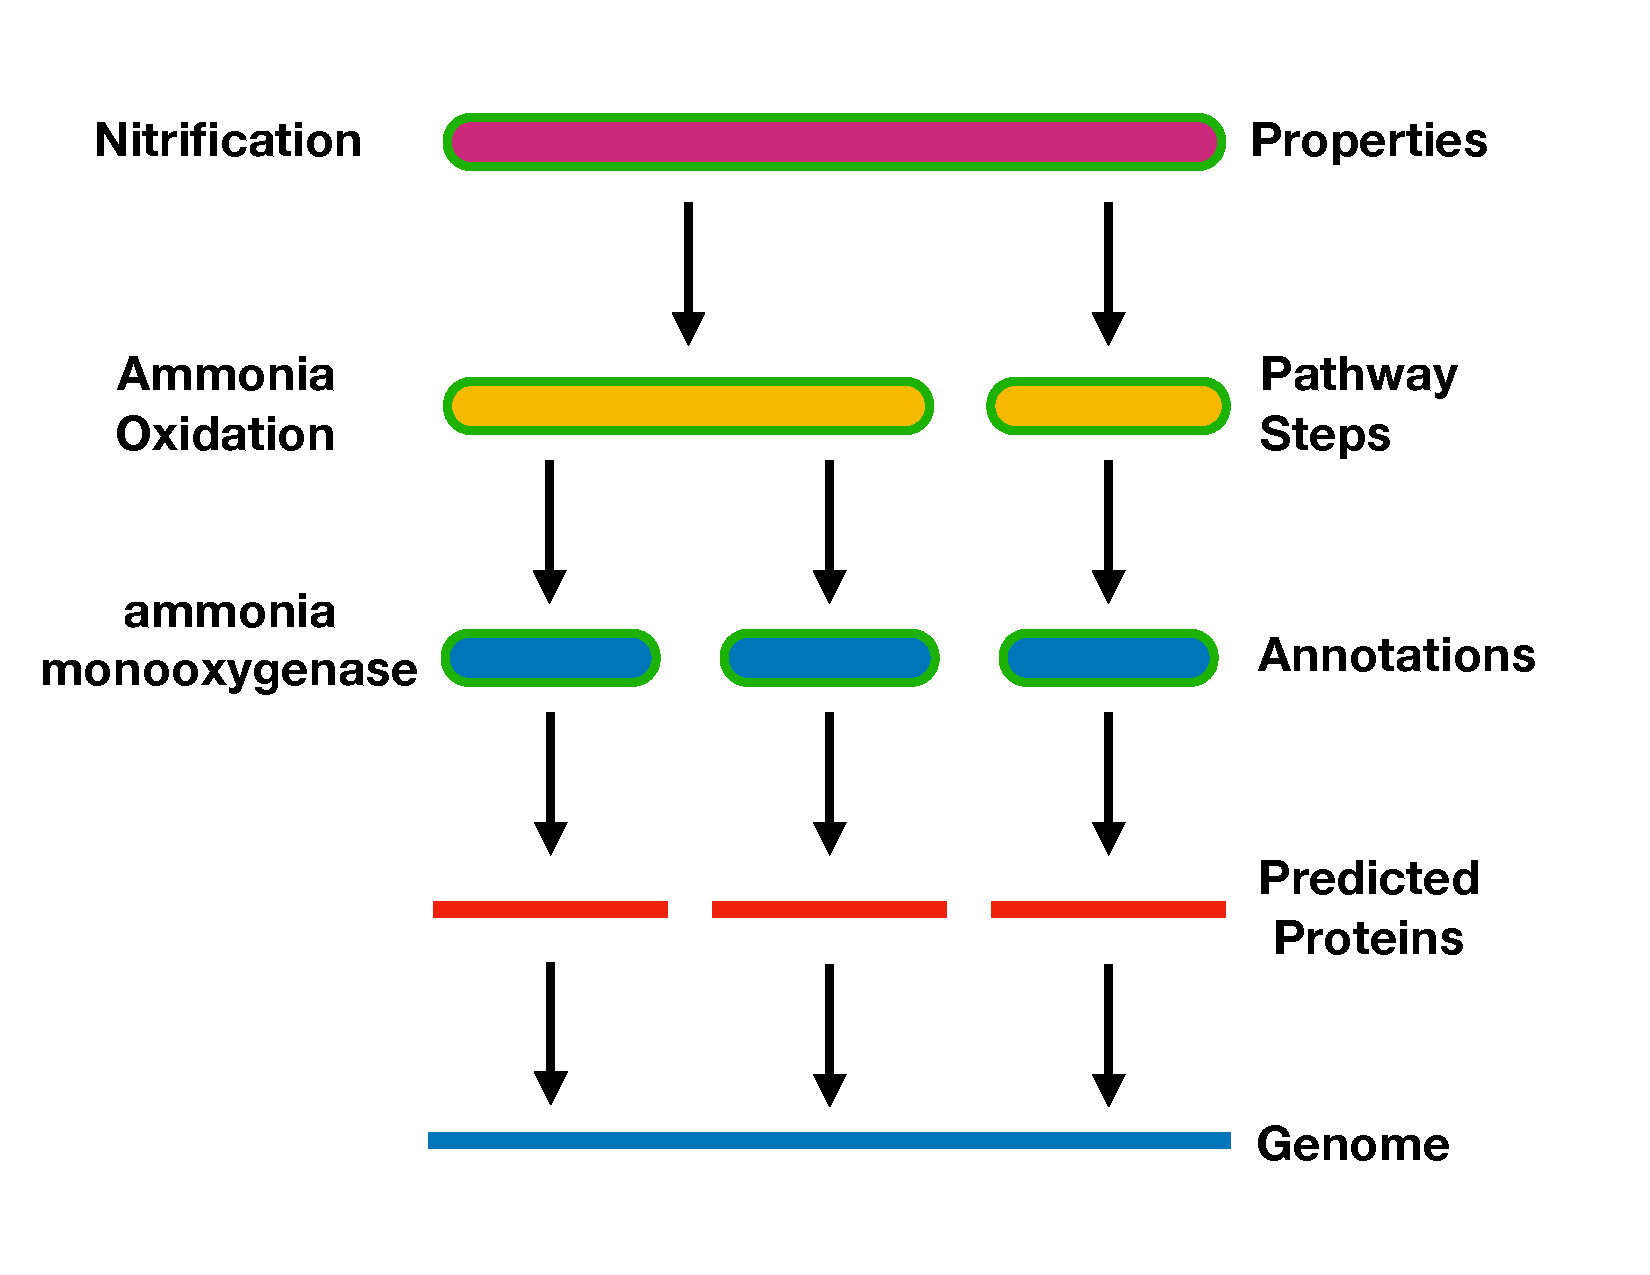
\includegraphics[width=0.9\textwidth]{media/pathway_analysis_steps.pdf}
	\caption[How the glyoxylate shunt can be predicted from the presence of its 
supporting enzymes.]{\textbf{How the glyoxylate shunt can be predicted from the 
presence of its supporting enzymes.}  If a microorganism is to be classified as 
possessing a glyoxylate shunt, then it should have highly similar proteins to 
those previously known to carry out the pathway, such as Iso and MalG. Several 
steps are required to go from an organism’s genome sequence to a prediction of 
its metabolic capabilities. The enzymes that carry out pathway steps must be 
identified (\textit{e}.\textit{g}., protein annotation). If found, they indicate 
the presence of pathway steps. Finally, if all or many steps are present, then 
the biochemical pathway can be said to be present.}
	 \label{fig:pathway-analysis-steps}
\end{figure}

\begin{figure}[!ht]
  \centering
	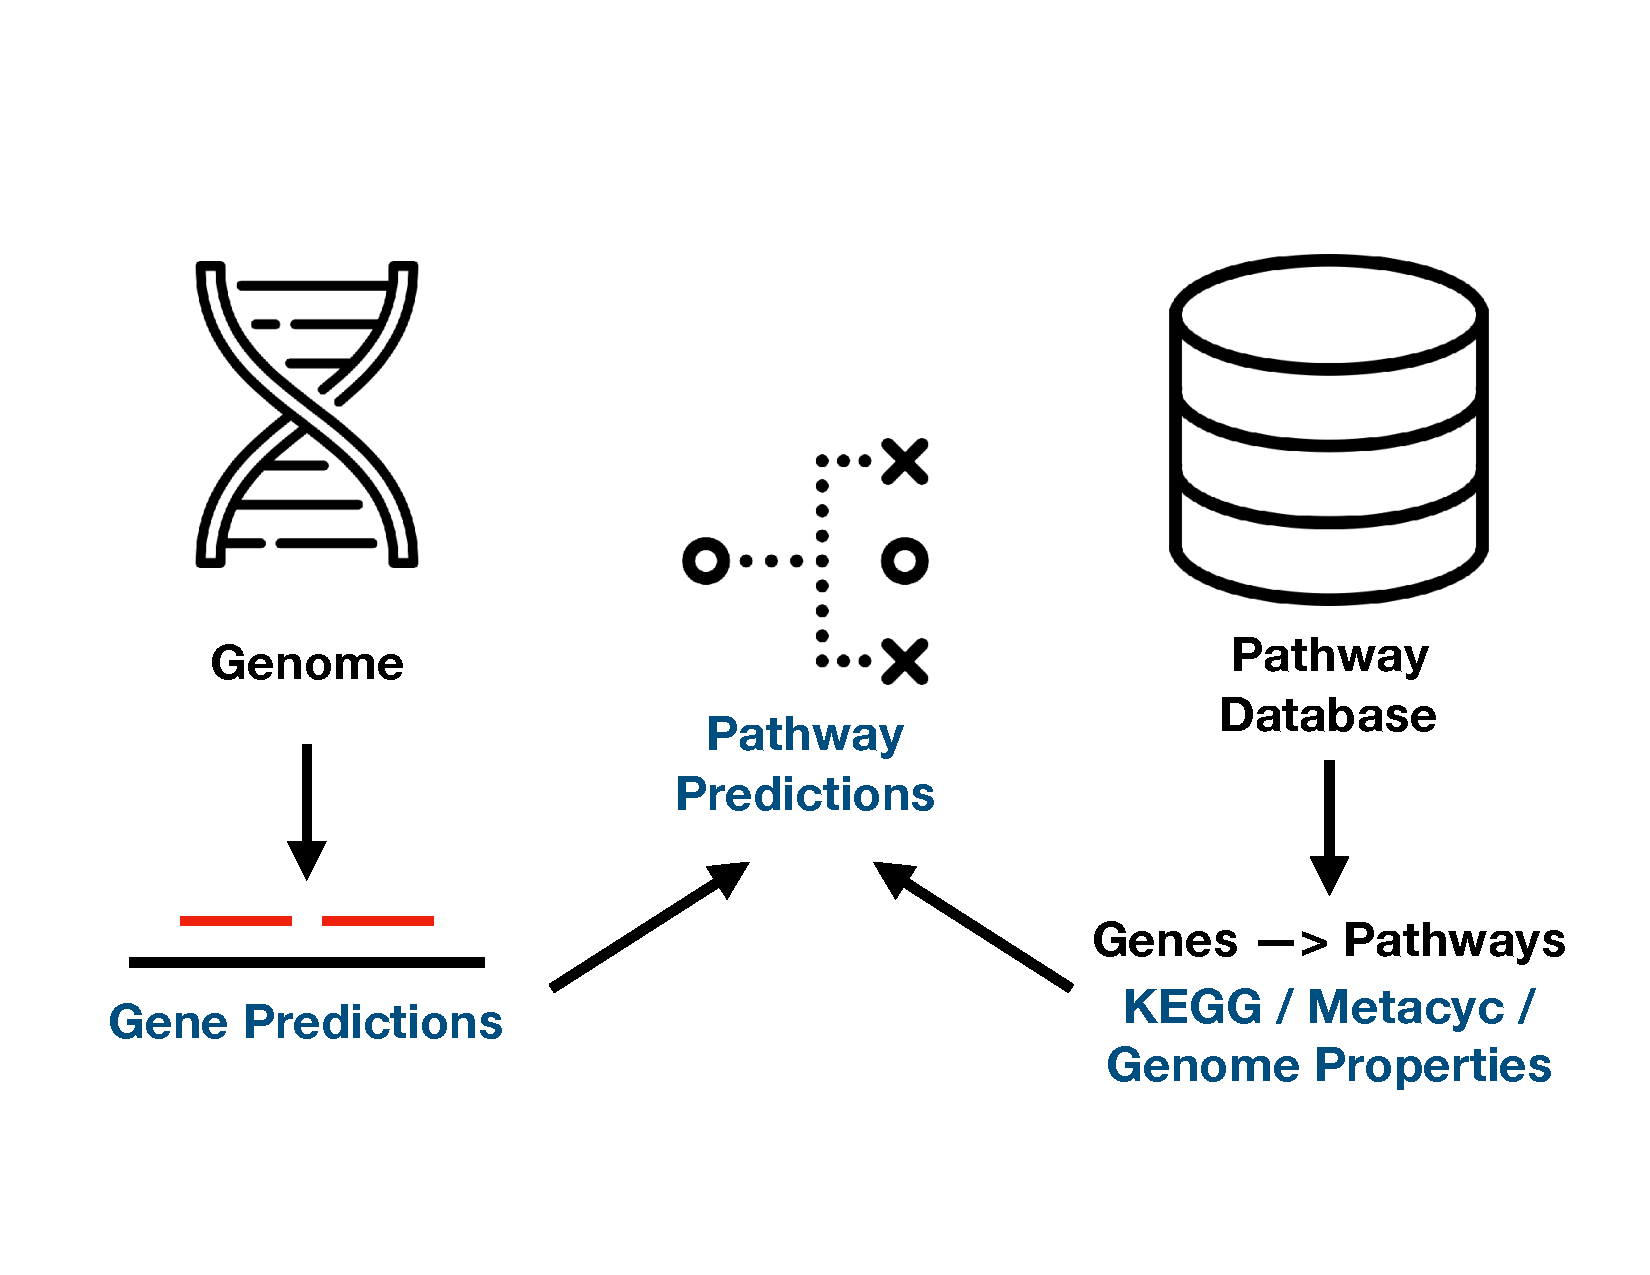
\includegraphics[width=0.8\textwidth]{media/pathway_bioinformatics.pdf}
	\caption[How an organism’s biochemical pathways are genomically predicted using 
information from pathway databases.]{\textbf{How an organism’s biochemical 
pathways are genomically predicted using information from pathway databases.} 
Predicting an organism’s biochemical pathways involves joining together two 
distinct datasets. One is a prediction of what genes are possessed by an 
organism. The other is a database containing the knowledge of what genes are 
involved in previously known biochemical pathways. When predicted proteins with 
sufficient homology to the previously cataloged genes are found within an 
organism’s genome, pathway prediction can be made.}
	 \label{fig:pathway-analysis-overview}
\end{figure}

Users can deploy pathway prediction bioinformatics pipelines in two ways. They 
can either be installed on to a user's computer, where genomes can be processed 
directly, or be deployed on to a web server, where users can upload their 
genomes for remote processing. Some pipelines only work with pathway data from a 
specific database. For example, Pathway Tools \cite{karp2002pathway} can only 
present information about pathways found within the MetaCyc 
\cite{karp2002metacyc} database. Often pipelines are optimized for generating 
data from the genomes of a specific clade on the tree of life. For example, 
Prokka \cite{seemann2014prokka}, a pipeline that predicts genes and annotates 
protein sequences, is only designed to work with the genomes of prokaryotic 
microbes. Prokka only carries out the first two steps of the key pathway 
analysis steps listed at the top of this section \cite{seemann2014prokka}. Once 
these proteins are predicted, they can be uploaded to servers such as \gls{kaas} 
\cite{moriya2007kaas} for pathway annotation. Several tools can perform all of the 
pathway analysis steps outlined in the key pathway analysis steps list. For 
example, \gls{rast} \cite{aziz2008rast} can take the upload of whole or partial 
bacterial genomes, predict the genes of these genomes, and provide users with a 
report displaying found pathways.

\section{The Current Bottlenecks of High Throughput Pathway Analysis}

Due to the current plethora of tools for genome annotation and pathway 
determination, identifying pathways for single organisms is becoming a solved 
problem. Researchers have progressed to comparing the presence and absence of 
pathways across organisms. Such comparisons are applied in order to, for 
example, find information about individual organism's ecological roles, 
evolution, or suitability towards different industrial tasks. For example, the 
genomes of organisms that are closely related phylogenetically could be compared 
to determine those that may have lost or gained a pathway or pathway step over 
time. Alternatively, the pathways possessed by multiple organisms from within 
the same environment could be compared to shed light on their potential 
ecological niches (Fig. \ref{fig:metagenomics}). Pathway comparisons could also 
be used industrially to select organisms to add to bioprocess co-cultures.

\begin{figure}[!ht]
  \centering
	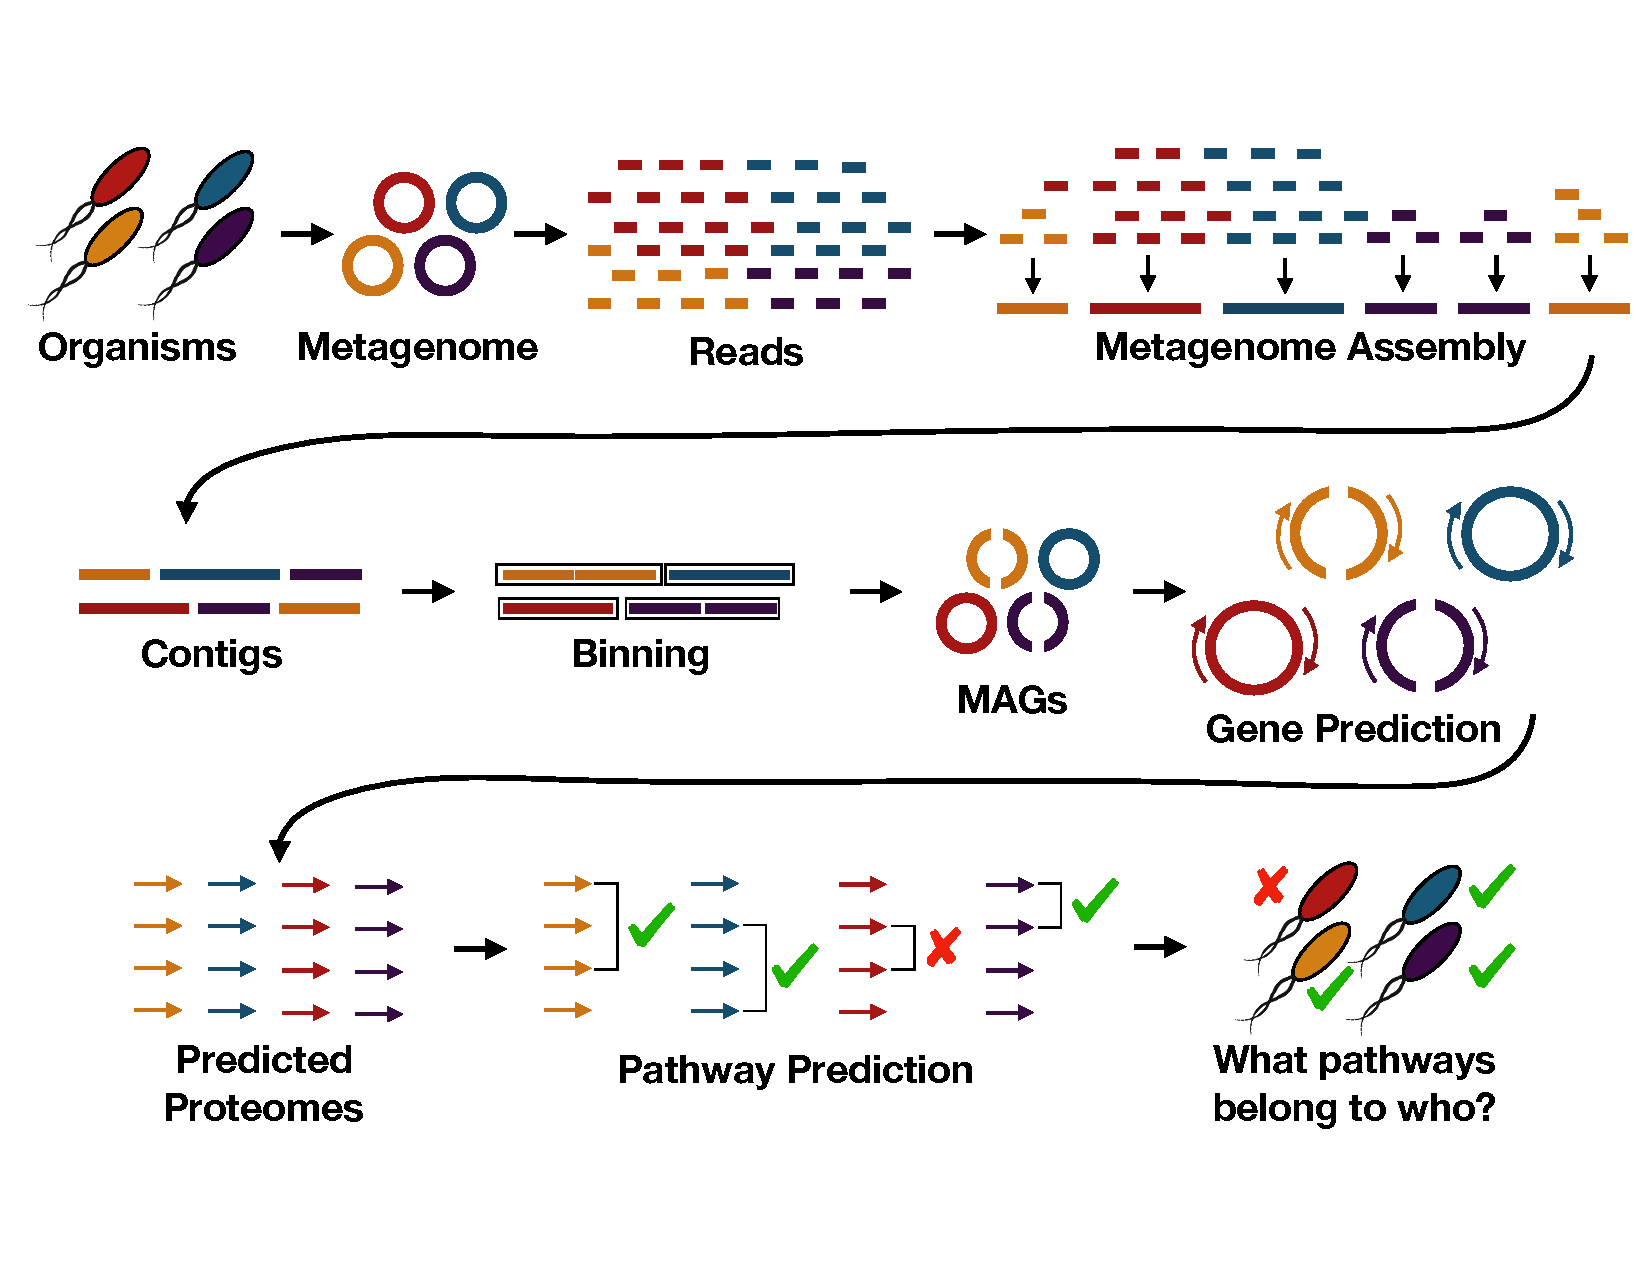
\includegraphics[width=0.75\textwidth]{media/metagenomics.pdf}
	\caption[Metagenomics steps used to determine the biochemical pathways 
possessed by organisms found in a single environment.]{\textbf{Metagenomics 
steps used to determine the biochemical pathways possessed by organisms found in 
a single environment.} Bioinformatics techniques can be used to separate 
individual genomes from a metagenomic sample. Pathway annotation can be 
performed on these genomes and used to compare the pathways possessed by 
different organisms from the same environment. Such comparisons can be used to 
evaluate each organism's potential role in an environment.}
	 \label{fig:metagenomics}
\end{figure}

Although assigning pathway presence and absence to individual organisms can be 
done quite rapidly, the comparison of these results across multiple organisms is 
currently a considerable bottleneck in the area of pathway analysis. Often 
pathway annotation tools that can process multiple genomes simultaneously 
present their results in the form of computer spreadsheets (\textit{e}.\textit{g}., Microsoft 
Excel or \gls{csv} files \cite{RFC4180}). After generation of these 
spreadsheets, users are required to manually scan through the thousands of 
pathway rows and organism columns to find pathway differences across organisms. 
Researchers with data science and coding skills may be able to generate custom R 
or Python scripts that assist them in this task by filtering down these 
spreadsheets to show only pathways that are different or by generating data 
visualizations that accelerate pattern detection. To accelerate script 
development, libraries have been written to help scriptwriters interact with 
pathway data. However, the majority of these libraries focus on helping users 
download data from existing pathway databases, rather than helping them with 
making comparisons across organisms. Thus, due to a lack of libraries for 
pathway comparison and lack of coding skills among biologists, there is a need 
for dedicated bioinformatics tools that simplify pathway comparisons across 
organisms. Software that visualizes the presence and absence of pathways 
would be of great use in this role. There are several emerging tools, which are 
discussed in Section \ref{micromeda-client-summary}, that help users visualize 
pathway annotations from multiple organisms. However, their implementation, in 
terms of visual idioms used and supporting data presented, is currently lacking. 
There is currently a gap for a tool that effectively presents such data and 
allows for rapid comparisons. There is also a gap for a pathway library that 
assists coders in making these comparisons programmatically. Finally, there is a 
gap for a tool that can both describe what pathways an organism possesses and 
allow users to identify the protein sequences that support these pathway 
annotations. Micromeda and Pygenprop were developed to fill these gaps.

\section{The Micromeda Platform} \label{micromeda-overview}

The bioinformatics system presented within this thesis, called Micromeda, is 
designed to address current gaps in the researcher's ability to compare pathway 
presence and absence across organisms. The platform does this without losing 
information about the protein sequences that support these pathways' existence. 
The output of the platform is an interactive heat map that displays rows of 
pathways by columns of organisms (Fig. \ref{fig:basic-heatmap-overview}). Heat 
map cells are coloured by the level of support for a pathway's existence in each 
genome (Fig. \ref{fig:basic-heatmap-overview}). This data visualization is 
displayed within a user's web browser. As discussed in Chapter 
\ref{micromeda-client}, this heat map is interactive, and users can tailor it to 
only display presence and absence for specific pathways or pathway steps. A 
software stack (see 
\href{http://en.wikipedia.org/wiki/Solution_stack}{en.wikipedia.org/wiki/Solution\_stack}) 
consisting of several components, some of which were developed as part of the 
thesis project, is used to generate data for the visualizations that Micromeda 
presents. This stack is outlined in the list below.

\begin{figure}[!ht]
  \centering
	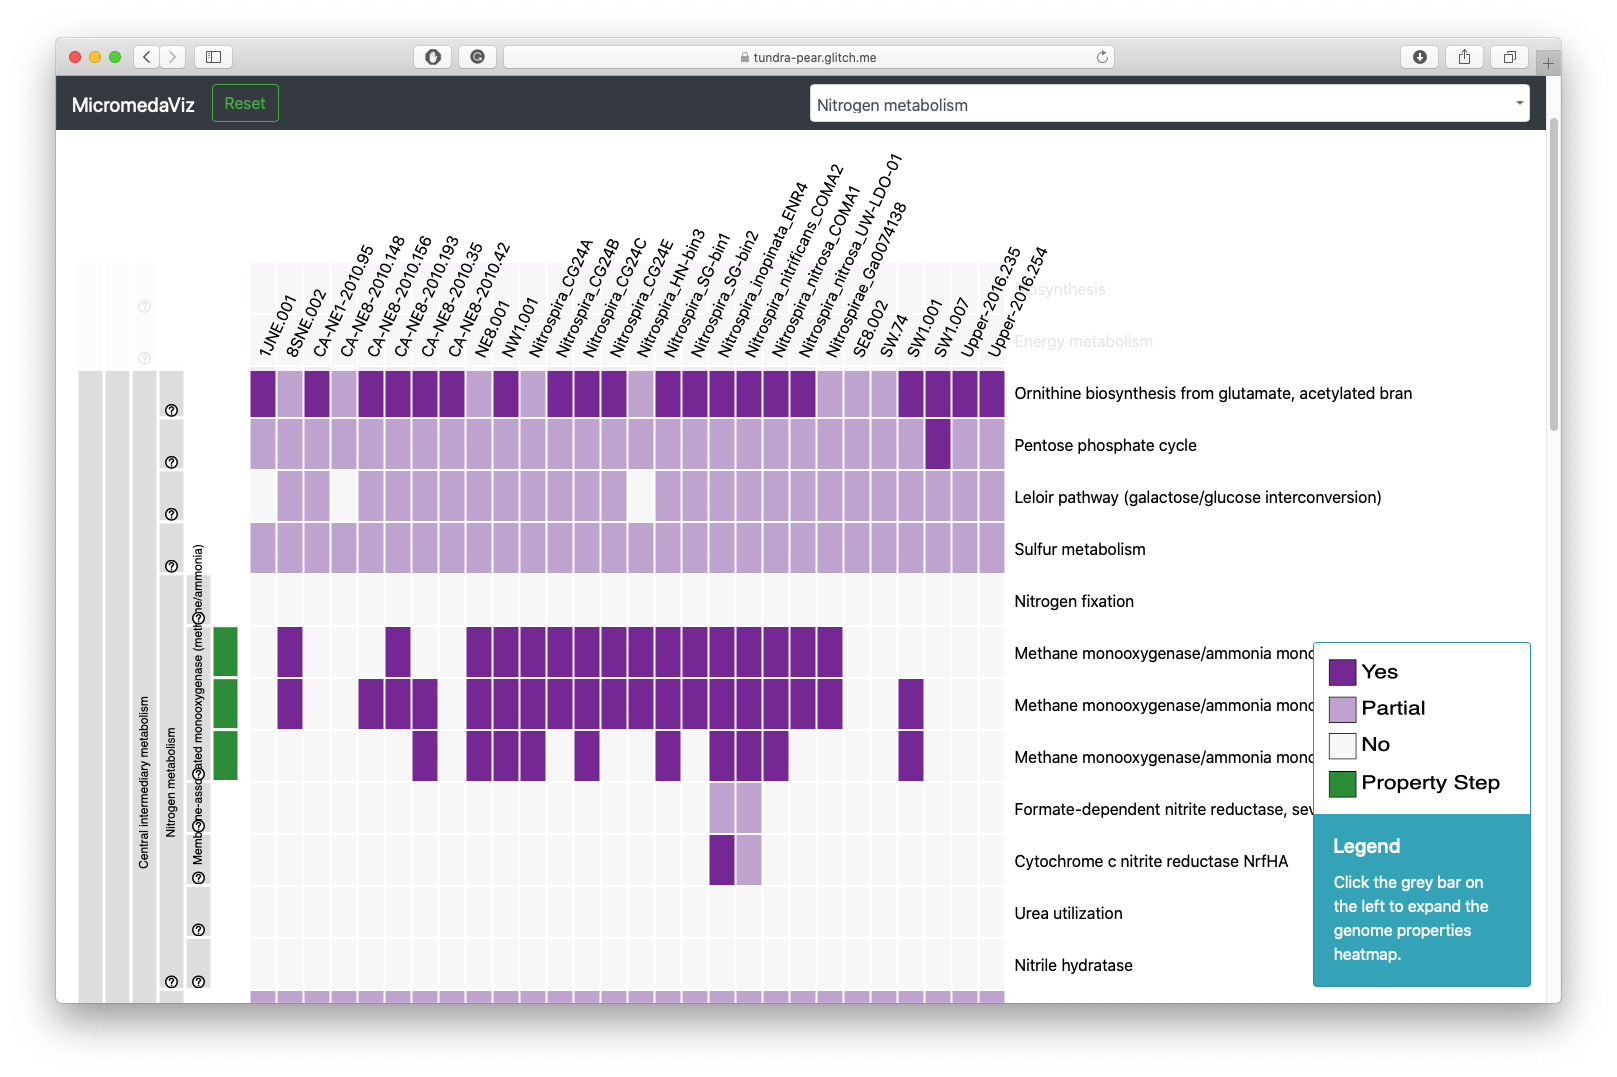
\includegraphics[width=0.9\textwidth]{media/Micromeda-Simple-Overview.png}
	 \caption[Web-browser window containing Micromeda’s heat map visualization 
and interface.] {\textbf{Web-browser window containing Micromeda’s heat map 
visualization and interface.} This heat map consists of pathway rows by organism 
columns and allows the comparison of pathway presence and absence across 
organisms. All other components of Micromeda were built to support this 
interface by providing it with data. Further explanation of the interface’s 
design can be found in Chapter \ref{micromeda-client}.}
	 \label{fig:basic-heatmap-overview}
\end{figure}

\begin{itemize}
\item A client web application that runs in the user's browser. This web 
application allows users to upload files to a server. These files contain 
precalculated data about an organism's predicted pathways and the protein 
sequences that support these predictions. This application draws pathway 
heat maps based on this uploaded data  (Fig. \ref{fig:basic-heatmap-overview}). 
These heat maps allow users to make comparisons across pathways and organisms. 
This component is called \textbf{Micromeda-Client} and is detailed in Chapter 
\ref{micromeda-client}. Links to a demonstration of the client interface can be 
found in Section \ref{client-demo}.
\item A server web application that runs on a remote computer system and in 
support of the client application. This server application accepts file uploads 
from the client and provides the client with easy access to the data held within 
the file. This component is called \textbf{Micromeda-Server} and is discussed in 
Chapter \ref{micromeda-server}.
\item A file format that allows users to easily transfer an assessment of what 
pathways are possessed by multiple organisms and the protein sequences used to 
support this assessment. These files, called \textbf{Micromeda files}, are the 
files uploaded to Micromeda-Server and use a custom format that is discussed in 
Section \ref{MicromedaFiles}. The format allows for the storage of the pathway 
and sequence information in the most compact way possible.
\item A software library that supports the generation of pathway annotations, 
rapid programmatic comparisons between organism pathway annotations and the 
generation of Micromeda files. The library is compatible with many 
emerging machine learning tools and opens up new avenues to their application to 
pathway analysis. This library is called \textbf{Pygenprop} and is discussed in 
Chapter \ref{Pygenprop}.
\item A pathway database that maps between predicted protein sequences derived 
from an organism's genome and biochemical pathway steps. The database chosen was 
the \textbf{Genome Properties} database \cite{richardson2018genome}. A short 
review of this database and the reason for its selection can be found in Chapter 
\ref{genome-properties}. This database is pre-existing and was not made as part 
of the thesis work.
\item A pre-existing sequence search program for scanning for identifying 
markers within the sequences of an organism's predicted proteins. These markers 
are used to identify enzymes that support the existence of a pathway. The search 
program chosen was \textbf{InterProScan5}, whose output data are used by the 
Genome Properties Database. An overview of InterProScan5 
\cite{jones2014interproscan} and its methodology can be found in Chapter 
\ref{genome-properties}.
\item A program that generates protein sequences from predicted genes found 
within an organism's genome. For example, in the case of prokaryotic genomes, an 
existing tool such as \textbf{Prodigal} \cite{hyatt2010prodigal} would be used. 
\end{itemize}


\begin{figure}[!ht]
  \centering
	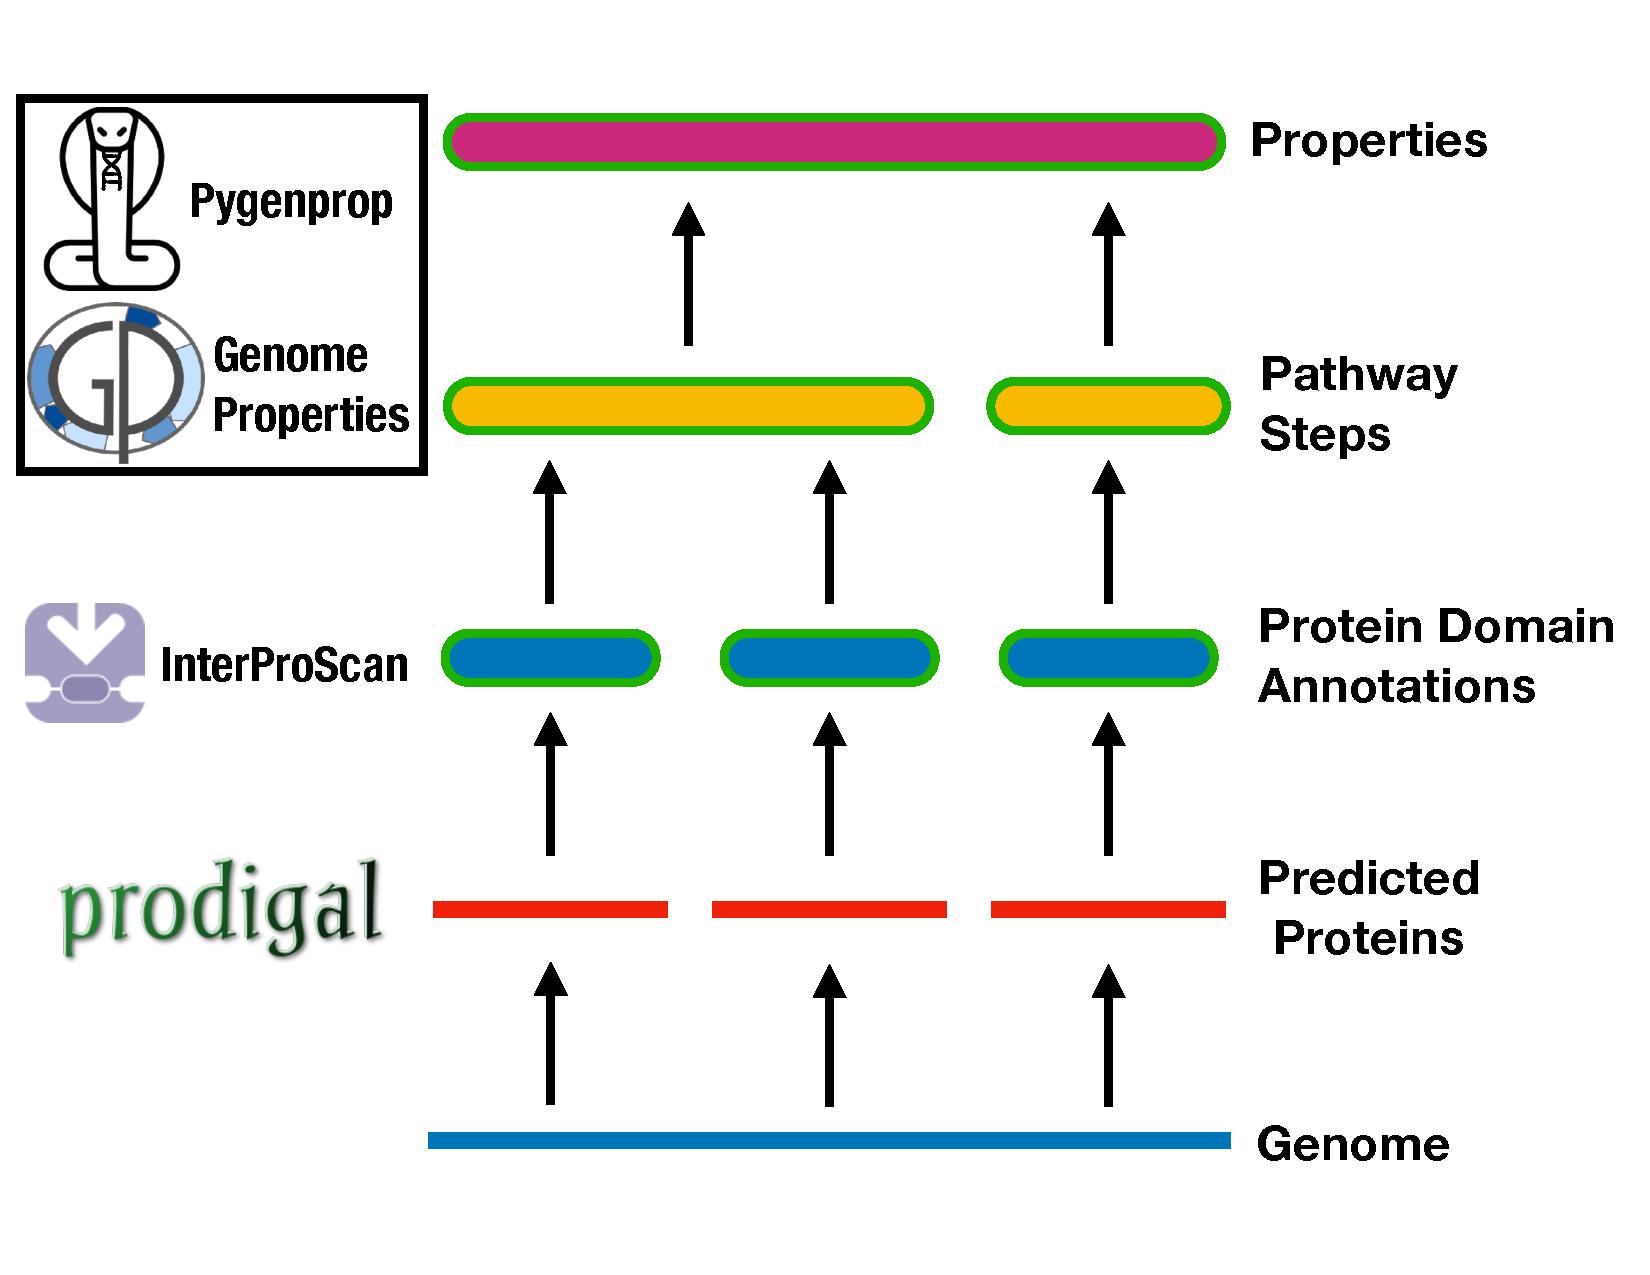
\includegraphics[width=0.8\textwidth]{media/micromeda-pipeline.pdf}
	 \caption[Steps performed and software tools used by Micromeda to predict the 
genome properties of an organism.]{\textbf{Steps performed and software tools 
used by Micromeda to predict the genome properties of an organism.} For 
prokaryotes, proteins must first be predicted via Prodigal. These proteins are 
then scanned using InterProScan5. The results of InterProScan are then combined 
with the Genome Properties database to predict pathways steps. These predictions 
are carried out by Pygenprop, which also predicts the overall presence and 
absence of pathways.}
	 \label{fig:micromeda-levels}
\end{figure}

\begin{figure}[!ht]
  \centering
	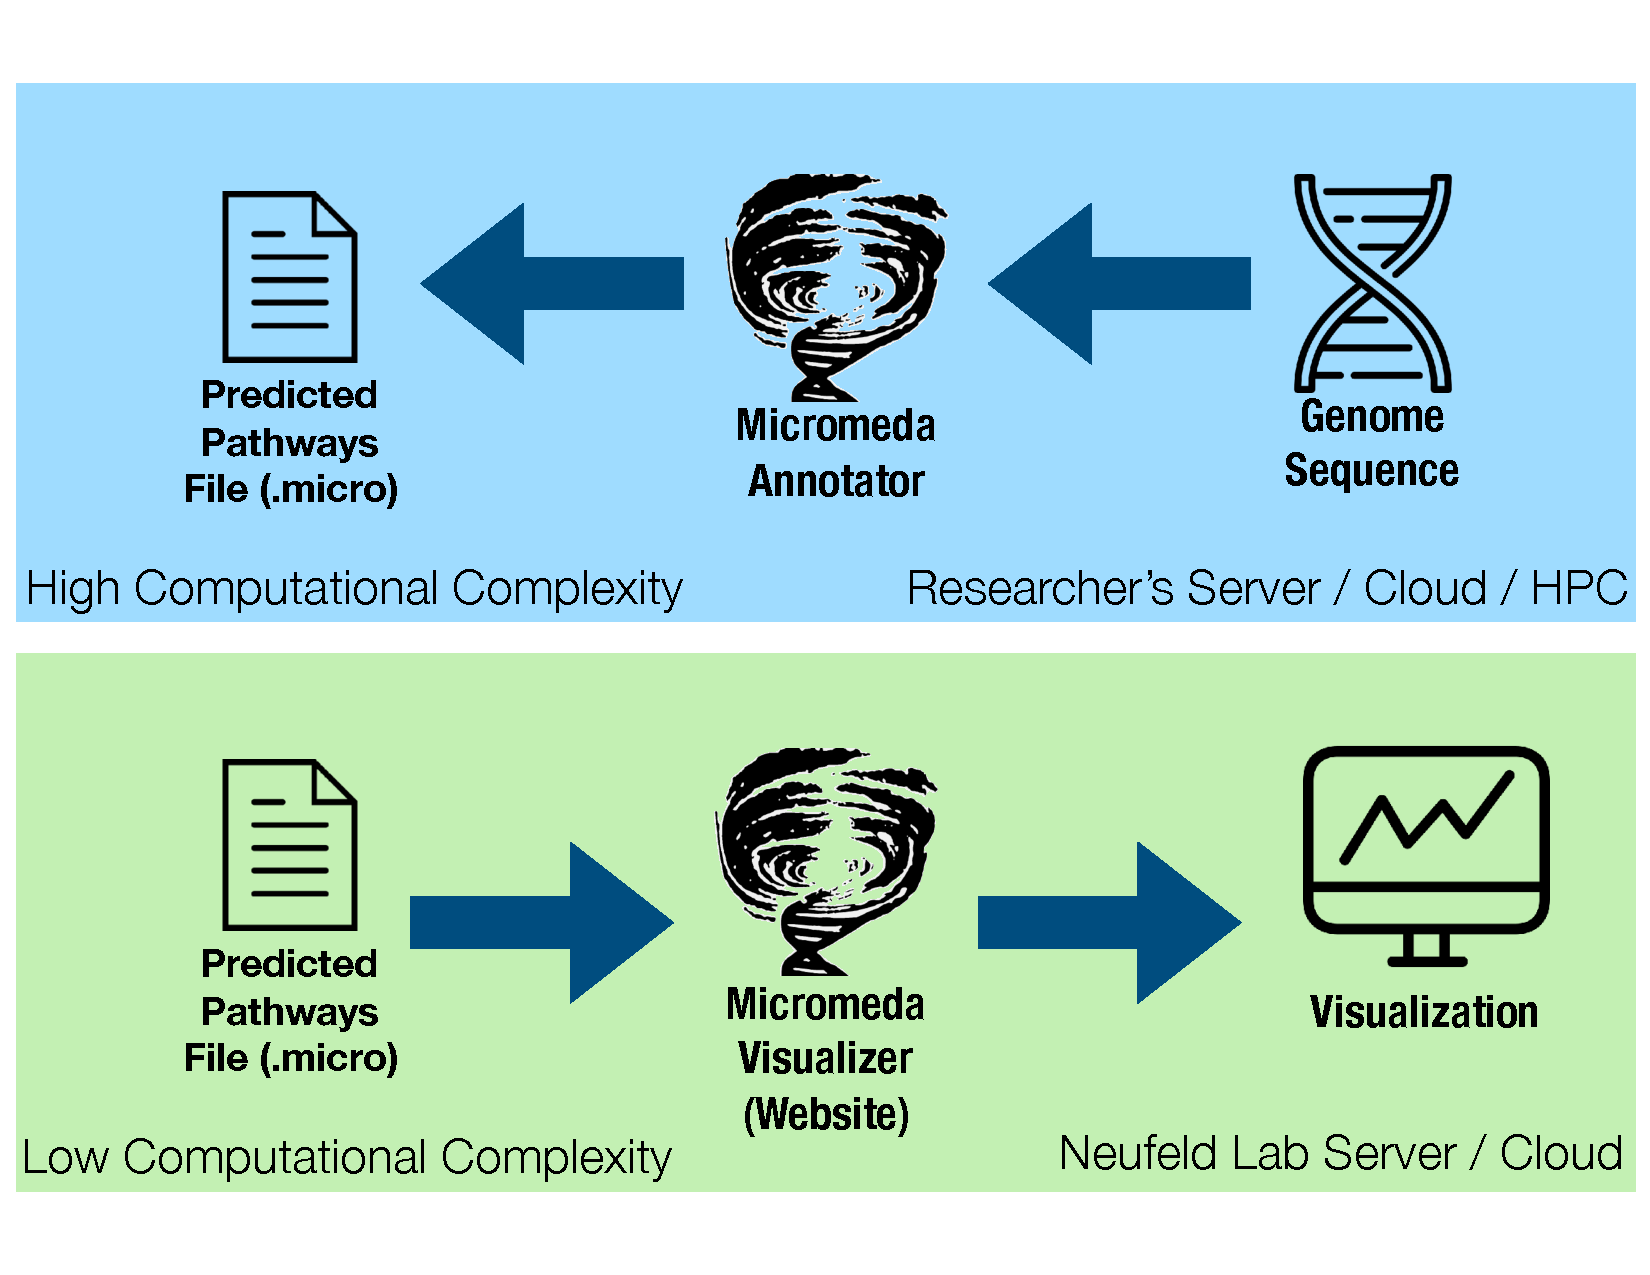
\includegraphics[width=0.8\textwidth]{media/micromeda-file-generation.pdf}
	 \caption[Two core steps that users must perform to generate Genome Properties 
visualizations using Micromeda.]{\textbf{Two core steps that users must perform 
to generate Genome Properties visualizations using Micromeda.} A local computer 
system must be used to execute a data generation step that creates a Micromeda 
file. Users can then upload this file to a second remote computer system that 
generates heat map visualizations. The most computationally complex step, 
Micromeda file generation, is not performed on the same server that generates 
the data visualizations.}
	 \label{fig:micromeda-file-generation}
\end{figure}

\begin{figure}[!ht]
  \centering
	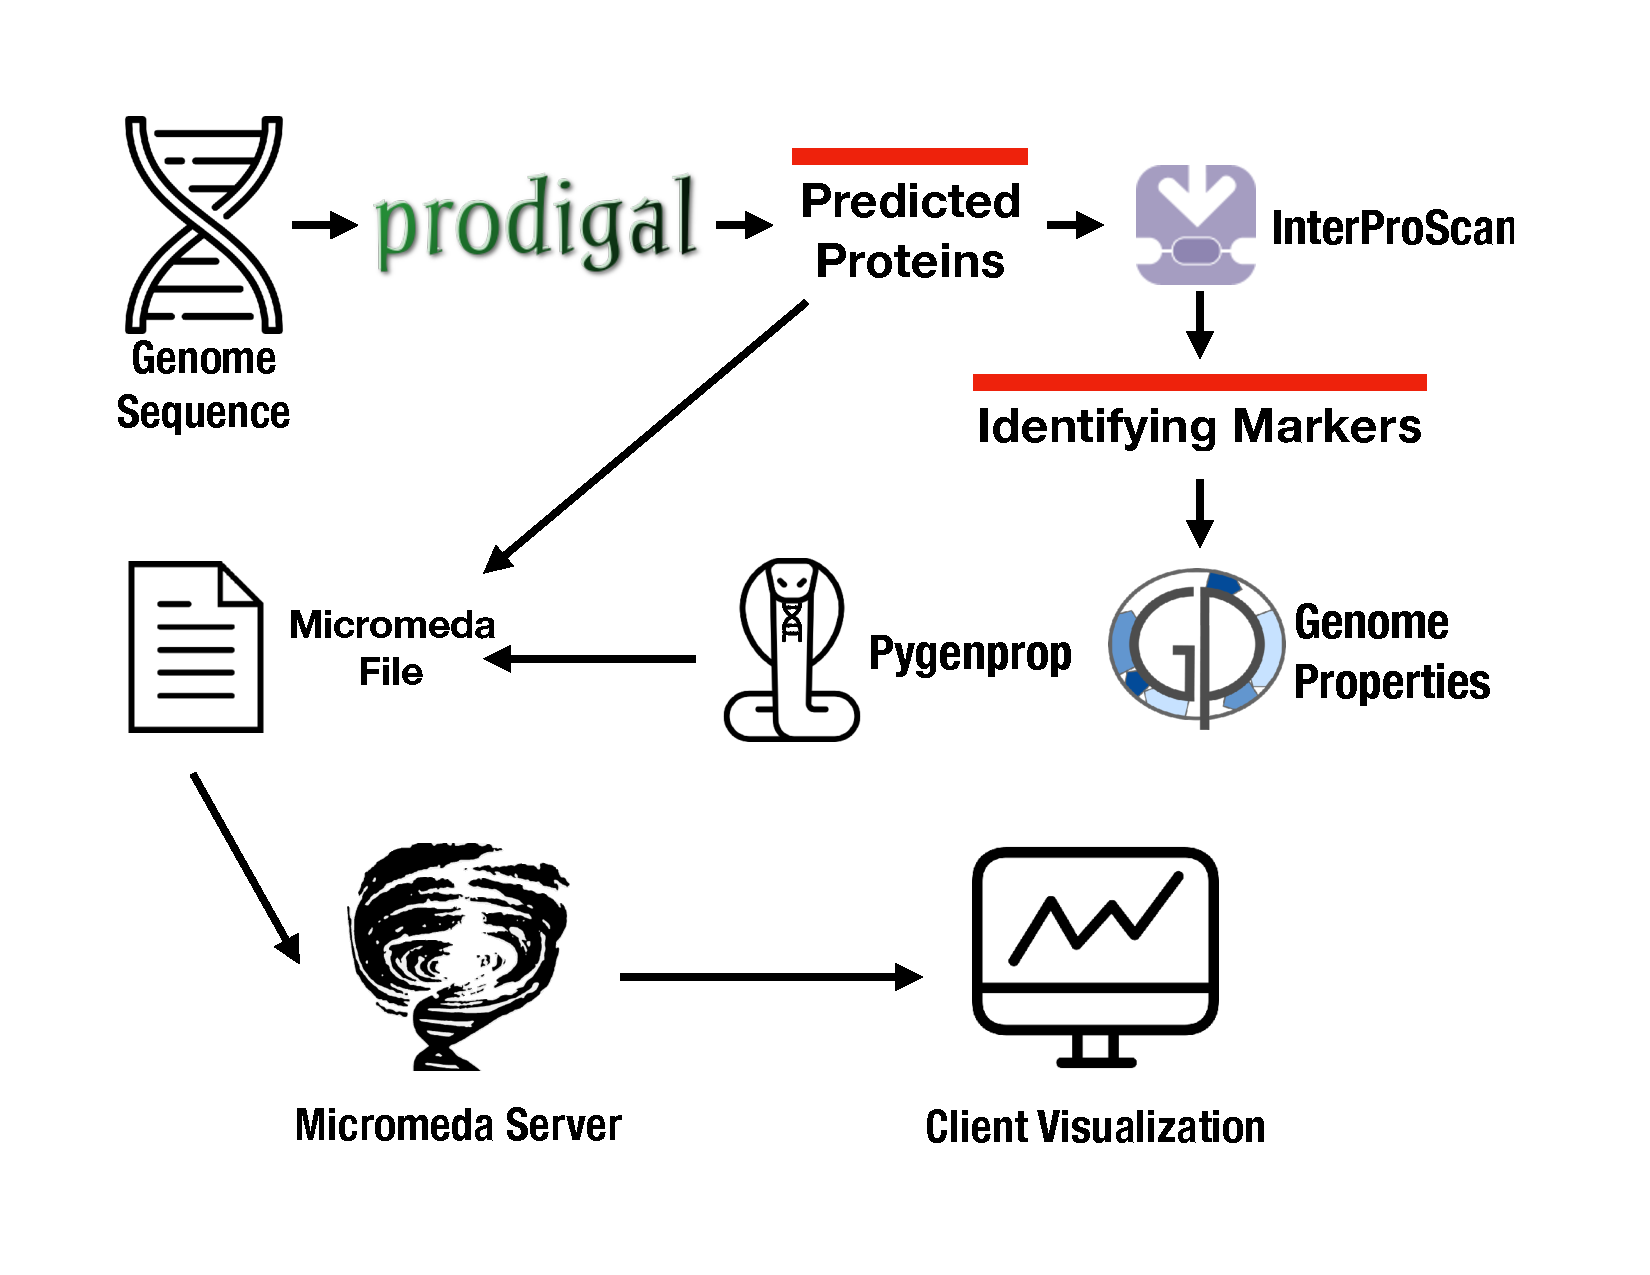
\includegraphics[width=0.8\textwidth]{media/how-micromeda-files-are-built.pdf}
	 \caption[How Micromeda files are built from InterProScan annotations of an 
organism's predicted proteins.]{\textbf{How Micromeda files are built from 
InterProScan annotations of an organism's predicted proteins.} These files 
possess not only pathway annotations but also the protein sequences that support 
them. Thus they allow for the transfer of complete pathway datasets. Micromeda 
files are uploaded to a remote server for visualization.}
	 \label{fig:micromeda-file-building-and-use}
\end{figure}

The Micromeda platform can be subdivided into two core components: a 
toolchain for generating Micromeda files (labelled Micromeda Annotator in Fig. 
\ref{fig:micromeda-file-generation}) and a web application for visualizing the 
data they contain (labelled Micromeda Visualizer in Fig. 
\ref{fig:micromeda-file-generation}). The individual steps for generating 
Micromeda files can be done manually using only three \gls{cli} tools (see Fig. 
\ref{fig:micromeda-levels}, Fig. \ref{fig:micromeda-file-building-and-use}, and  
\href{http://en.wikipedia.org/wiki/Command-line_interface}{en.wikipedia.org/wiki/Command-line\_interface}). 
For example, with prokaryotic genomes, Prodigal could be used to predict protein 
sequences from an organism's genome sequence, and InterProScan5 could be used to 
scan these proteins to identify enzymes that support the existence of specific 
pathways (Fig. \ref{fig:micromeda-file-building-and-use}). Afterwards, a short 
Python script, built using the Pygenprop library, could be used to convert the 
output from InterProScan and Prodigal into a single Micromeda file. This script 
would also use a copy of the Genome Properties database (Fig. 
\ref{fig:micromeda-file-building-and-use}). An example of such a script can be 
found within Pygenprop's GitHub repository 
(\href{http://github.com/Micromeda/pygenprop}{github.com/Micromeda/pygenprop}). 
An explicit automated software pipeline for generating Micromeda files does not 
currently exist. However, its potential implementation is discussed in 
Subsection \ref{pipeline-development}.


\subsection{Software Architecture Overview}

Micromeda follows a client-server web architecture \cite{svobodova1985client} 
(see 
\href{http://en.wikipedia.org/wiki/Client-server_model}{en.wikipedia.org/wiki/Client-server\_model} 
and Section \ref{web-servers}). Users interact with Micromeda-Client via their 
web browser, and this client allows them to upload Micromeda files to 
Micromeda-Server. Micromeda files contain all the information that the client 
requires to generate a pathway heat map. These files store pathway annotations, 
InterProScan5 output data, and supporting protein sequences for multiple 
organisms (see Section \ref{MicromedaFiles}). Having all these datasets in a 
single file simplifies the data upload process as only one file has to be 
uploaded by the user per heat map drawn. After upload, the contents of the 
uploaded file are stored temporarily in \gls{ram} on the computer used to host 
Micromeda-Server (see Section \ref{server-workflow}). Micromeda-Client will ask 
Micromeda-Server for data from this file as the client draws a heat map or 
responds to user activity (see Section \ref{client-implementation}). Multiple 
users can interact with Micromeda-Server and Client simultaneously.

\subsection{The Reasoning for Building a Web Application and Having Micromeda 
files} \label{why-micromeda-files}

Micromeda's \gls{ui} runs inside a user's web browser. The reasoning for using 
this approach, in contrast to building Micromeda as a native desktop 
application, is discussed in Section \ref{client-delivery-method}. The reason 
Micromeda files exist is that they allow the rapid transfer of pathway 
annotation datasets that, in turn, allow for a separation of data generation and 
visualization. This separation is essential because there are vast computational 
complexity differences between creating pathway annotations and visualizing 
their contents. Micromeda's pathway prediction method involves identifying 
specific enzymes by running InterProScan5 on the set of all predicted proteins 
of an organism. The algorithms used by InterProScan5 are very computationally 
complex. It takes on the order of two hours to scan through the 4313 proteins of 
\textit{E. coli} K12 (\gls{ncbitaxa}: 1010810) using 100\% of all the \gls{cpu} 
cores of a 16 core server\footnote{InterProScan5 was tested on a server with two 
Intel E5310 (4 \gls{cpu} cores/4 threads/8 \gls{mb} cache/1.60 \gls{ghz} clock 
speed) processors and 16 \gls{gb}  of \gls{ram}.}.

In contrast, Micromeda can render a pathway heat map for over forty organisms in 
less than a second. Thus, if one wanted to have a web application that both 
computes and visualizes pathway annotations for uploaded genome sequences, then 
this application would require the support of an extensive and well-maintained 
hardware infrastructure. Developing the code to build, maintain, and sustain 
such a system draws away from the core goal of the Micromeda platform, which was 
to design a tool that helps users visualize pathway differences across 
organisms. Hence, for Micromeda, I chose to have users generate pathway 
annotations locally, using InterProScan5 and other tools, and have them upload 
these files to a remote web server for visualization (Fig. 
\ref{fig:micromeda-file-generation}). This design decision significantly reduces 
the hardware requirements for those who want to host Micromeda-Server and 
Client. The decision also reduces the overall design complexity of 
Micromeda-Client and Server and allows future development to focus on creating 
better and more feature-rich versions of Micromeda's \gls{ui} and 
visualizations.

\section{Summary} \label{introduction_summary}

Micromeda allows users to visualize the differences in pathway presence and 
absence across organisms. The tool does this based on the data contained within 
uploaded Micromeda files. Pygenprop is a software library that can not only 
produce Micromeda files but also make programmatic comparisons of pathway 
presence and absence across organisms. Potential improvements to individual 
components of Micromeda are highlighted in the summary section of each of their 
chapters. Potential improvements that would require modification of multiple 
components are highlighted in Chapter \ref{conclusion-chapter}. As discussed in 
Chapter \ref{conclusion-chapter}, Micromeda breaks new ground in both features 
and implementation and will increase both the speed and ease at which 
researchers perform pathway analysis.

%======================================================================
\chapter{Observations}
%======================================================================

This would be a good place for some figures and tables.

Some notes on figures and photographs\ldots

\begin{itemize}
\item A well-prepared PDF should be 
  \begin{enumerate}
    \item Of reasonable size, {\it i.e.} photos cropped and compressed.
    \item Scalable, to allow enlargment of text and drawings. 
  \end{enumerate} 
\item Photos must be bit maps, and so are not scaleable by definition. TIFF and
BMP are uncompressed formats, while JPEG is compressed. Most photos can be
compressed without losing their illustrative value.
\item Drawings that you make should be scalable vector graphics, \emph{not} 
bit maps. Some scalable vector file formats are: EPS, SVG, PNG, WMF. These can
all be converted into PNG or PDF, that pdflatex recognizes. Your drawing 
package probably can export to one of these formats directly. Otherwise, a 
common procedure is to print-to-file through a Postscript printer driver to 
create a PS file, then convert that to EPS (encapsulated PS, which has a 
bounding box to describe its exact size rather than a whole page). 
Programs such as GSView (a Ghostscript GUI) can create both EPS and PDF from PS files.
Appendix~\ref{AppendixA} shows how to generate properly sized Matlab plots and save them as PDF.
\item It's important to crop your photos and draw your figures to the size that
you want to appear in your thesis. Scaling photos with the 
includegraphics command will cause loss of resolution. And scaling down 
drawings may cause any text annotations to become too small.
\end{itemize}

For more information on \LaTeX\, see the uWaterloo Skills for the Academic Workplace  \href{https://uwaterloo.ca/information-systems-technology/services/electronic-thesis-preparation-and-submission-support/ethesis-guide/creating-pdf-version-your-thesis/creating-pdf-files-using-latex/latex-ethesis-and-large-documents}{course notes}. 
\footnote{
Note that while it is possible to include hyperlinks to external documents,
it is not wise to do so, since anything you can't control may change over time. 
It \emph{would} be appropriate and necessary to provide external links to 
additional resources for a multimedia ``enhanced'' thesis. 
But also note that if the \package{hyperref} package is not included, 
as for the print-optimized option in this thesis template, any \cmmd{href} 
commands in your logical document are no longer defined.
A work-around employed by this thesis template is to define a dummy \cmmd{href} 
command (which does nothing) in the preamble of the document, 
before the \package{hyperref} package is included. 
The dummy definition is then redifined by the
\package{hyperref} package when it is included.
}

The classic book by Leslie Lamport \cite{lamport.book}, author of \LaTeX , is worth a look too, and the many available add-on packages are described by 
Goossens \textit{et al} \cite{goossens.book}.

%----------------------------------------------------------------------
% END MATERIAL
% Bibliography, Appendices, Index, etc.
%----------------------------------------------------------------------

% Bibliography

% The following statement selects the style to use for references.  It controls the sort order of the entries in the bibliography and also the formatting for the in-text labels.
\bibliographystyle{plain}
% This specifies the location of the file containing the bibliographic information.  
% It assumes you're using BibTeX to manage your references (if not, why not?).
\cleardoublepage % This is needed if the book class is used, to place the anchor in the correct page,
                 % because the bibliography will start on its own page.
                 % Use \clearpage instead if the document class uses the "oneside" argument
\phantomsection  % With hyperref package, enables hyperlinking from the table of contents to bibliography             
% The following statement causes the title "References" to be used for the bibliography section:
\renewcommand*{\bibname}{References}

% Add the References to the Table of Contents
\addcontentsline{toc}{chapter}{\textbf{References}}

\bibliography{uw-ethesis}
% Tip 5: You can create multiple .bib files to organize your references. 
% Just list them all in the \bibliogaphy command, separated by commas (no spaces).

% The following statement causes the specified references to be added to the bibliography% even if they were not 
% cited in the text. The asterisk is a wildcard that causes all entries in the bibliographic database to be included (optional).
\nocite{*}
%----------------------------------------------------------------------

% Appendices

% The \appendix statement indicates the beginning of the appendices.
\appendix
% Add a title page before the appendices and a line in the Table of Contents
\chapter*{APPENDICES}
\addcontentsline{toc}{chapter}{APPENDICES}
% Appendices are just more chapters, with different labeling.
\chapter[PDF Plots From Matlab]{Matlab Code for Making a PDF Plot}
\label{AppendixA}
% Tip 4: Example of how to get a shorter chapter title for the Table of Contents 
%======================================================================
\section{Using the Graphical User Interface}
Properties of Matab plots can be adjusted from the plot window via a graphical interface. Under the Desktop menu in the Figure window, select the Property Editor. You may also want to check the Plot Browser and Figure Palette for more tools. To adjust properties of the axes, look under the Edit menu and select Axes Properties.

To set the figure size and to save as PDF or other file formats, click the Export Setup button in the figure Property Editor.

\section{From the Command Line} 
All figure properties can also be manipulated from the command line. Here's an example: 
\begin{verbatim}
x=[0:0.1:pi];
hold on % Plot multiple traces on one figure
plot(x,sin(x))
plot(x,cos(x),'--r')
plot(x,tan(x),'.-g')
title('Some Trig Functions Over 0 to \pi') % Note LaTeX markup!
legend('{\it sin}(x)','{\it cos}(x)','{\it tan}(x)')
hold off
set(gca,'Ylim',[-3 3]) % Adjust Y limits of "current axes"
set(gcf,'Units','inches') % Set figure size units of "current figure"
set(gcf,'Position',[0,0,6,4]) % Set figure width (6 in.) and height (4 in.)
cd n:\thesis\plots % Select where to save
print -dpdf plot.pdf % Save as PDF
\end{verbatim}

%----------------------------------------------------------------------
\end{document} % end of logical document
